\chapter{Волны, квантованные моды и операторы рождения}

\section{Волны, поля и комплексные экспоненты}

Квантовая теория поля — основной инструмент физики элементарных частиц. Прежде чем давать даже элементарное изложение квантового поля, полезно собрать математические факты, связывающие волны с частицами. Волна уже является конфигурацией поля: поле меняется от точки к точке в пространстве, а волна — это конфигурация, в которой эти значения осциллируют и распространяются. Квантовая механика даёт связь между такими волнами и частицами.

Здесь предполагается, что квантовая механика и специальная теория относительности уже известны. Непосредственная цель состоит в том, чтобы повторить элементы, необходимые для физики элементарных частиц, а не заменить курс по любой из этих дисциплин.

Экспонента характеризуется пропорциональным ростом. Если
\begin{equation}
f(x)=e^{\alpha x},
\end{equation}
то
\begin{equation}
\frac{df}{dx}=\alpha f.
\end{equation}
На малом интервале приращение пропорционально уже имеющемуся количеству. Наглядный пример даёт популяция, растущая в чашке Петри: чем больше организмов уже имеется, тем больше их доступно для размножения, так что скорость роста пропорциональна самой популяции. Умножение \(e^{\alpha x}\) на общий постоянный множитель не меняет этого определяющего свойства.

Синус и косинус не растут, а колеблются. Это одна и та же кривая, сдвинутая на четверть периода, и дифференцирование переводит их друг в друга:
\begin{align}
\frac{d}{dx}\sin(kx)&=k\cos(kx),\\
\frac{d}{dx}\cos(kx)&=-k\sin(kx).
\end{align}
Ни одна из этих функций сама по себе не является экспонентой, потому что её производная пропорциональна другой функции. Однако их комплексная комбинация обладает экспоненциальным свойством. При \(i^2=-1\),
\begin{align}
\frac{d}{dx}\bigl(\cos(kx)+i\sin(kx)\bigr)
&=-k\sin(kx)+ik\cos(kx)\\
&=ik\bigl(\cos(kx)+i\sin(kx)\bigr).
\end{align}
Следовательно,
\begin{equation}
e^{ikx}=\cos(kx)+i\sin(kx).
\end{equation}
Это тождество возникает снова и снова, потому что синусы и косинусы описывают волнообразные колебания. Когда \(x\) — пространственная координата, функция колеблется в пространстве. Когда аргументом является время, она колеблется во времени.

\section{Частота, длина волны и импульс фотона}

Обычная частота \(f\) — это число полных циклов в секунду. Цикл означает одно полное колебание. Угловая частота описывает то же движение в радианах в секунду:
\begin{equation}
\omega=2\pi f.
\end{equation}
Эти два обозначения описывают одну и ту же частоту. Между ними переходят, чтобы не загромождать вычисление лишними множителями \(2\pi\), хотя полностью эти множители никогда не исчезают.

Длина волны \(\lambda\) — это расстояние, занимаемое одним полным пространственным циклом. Если волна распространяется со скоростью \(v\), то расстояние на цикл, умноженное на число циклов в секунду, даёт скорость распространения:
\begin{equation}
\lambda f=v.
\end{equation}
Для света в вакууме \(v=c\), поэтому
\begin{equation}
\lambda f=c.
\end{equation}
Для звуковой волны правая часть — это скорость звука, а для волны на воде — соответствующая скорость водной волны. Поэтому появление \(c\) — это утверждение о свете, а не определение, общее для всякой волны.

В квантовой механике постоянная Планка вводится в двух обозначениях,
\begin{equation}
\hbar=\frac{h}{2\pi}.
\end{equation}
Переход от \(h\) к \(\hbar\) лишь переносит множители \(2\pi\) из одного уравнения в другое.

Численные значения размерных констант зависят от единиц, в которых их выражают. Метры, секунды и килограммы — условности человеческого масштаба, удобные для обычных длин и времён. Традиционные единицы, сопоставимые с длиной руки, были удобны для ткани или верёвки; каков бы ни был точный исторический путь к метру, никакой фундаментальный принцип не выделяет именно этот человеческий масштаб. В единицах СИ,
\begin{equation}
\begin{aligned}
h &\simeq 6.6\times10^{-34}\ \mathrm{J\,s},
&\hbar &\simeq 1.1\times10^{-34}\ \mathrm{J\,s},\\
c &\simeq 3\times10^8\ \mathrm{m\,s^{-1}}.
\end{aligned}
\end{equation}
Смысл этих чисел — в их масштабе в обычных единицах: постоянная Планка чрезвычайно мала, а скорость света чрезвычайно велика.

Один квант моды имеет энергию
\begin{equation}
E_{\text{one quantum}}=\hbar\omega=hf.
\end{equation}
Это энергия одного фотона, а не полная энергия произвольной классической электромагнитной волны. Видимый свет имеет частоту порядка \(10^{15}\) циклов в секунду, поэтому типичный оптический фотон имеет энергию порядка
\begin{equation}
E_\gamma\sim 10^{-19}\ \mathrm{J}.
\end{equation}
Даже столь быстрое оптическое колебание даёт очень малую энергию на квант, потому что \(h\) столь мала. Поэтому макроскопическое количество оптической энергии содержит огромное число фотонов.

Энергия и импульс заслуживают особого внимания, поскольку обе эти величины сохраняются. Это удобные величины для учёта: полная энергия и импульс, входящие в процесс, должны уравновешиваться полной энергией и импульсом, выходящими из него. Импульс — вектор и направлен по движению. Для частицы, движущейся намного медленнее света,
\begin{equation}
\vec p=m\vec v.
\end{equation}

Рассмотрим теперь электромагнитное излучение, коллимированное вдоль одного направления, а не распределённое по многим направлениям. Его импульс направлен вдоль пучка. Нерелятивистскую формулу нельзя применять к фотону, потому что \(m\) означает массу покоя, а фотон имеет нулевую массу покоя. Тем не менее существует полезная размерностная подсказка. Если \emph{неправомерно} приписать фотону величину \(E/c^2\), как если бы это была масса, а затем подставить \(v=c\), получится
\begin{equation}
mv\longrightarrow \frac{E}{c^2}c=\frac{E}{c}.
\end{equation}
Этот приём случайно даёт правильный ответ и правильные единицы, но не является корректным доводом в пользу того, что фотон имеет массу покоя \(E/c^2\). Правильное релятивистское соотношение для коллимированного излучения имеет вид
\begin{equation}
|\vec p|=\frac{E}{c}.
\end{equation}
Уравнение даёт модуль. Направление — то, в котором распространяется излучение.

Для одного фотона,
\begin{align}
|\vec p_\gamma|
&=\frac{E_\gamma}{c}
=\frac{hf}{c}.
\end{align}
Для света,
\begin{equation}
\lambda f=c,
\qquad
\frac{f}{c}=\frac{1}{\lambda},
\end{equation}
и поэтому
\begin{equation}
|\vec p_\gamma|=\frac{hf}{c}=\frac{h}{\lambda}.
\end{equation}

\begin{figure}[t]
\centering
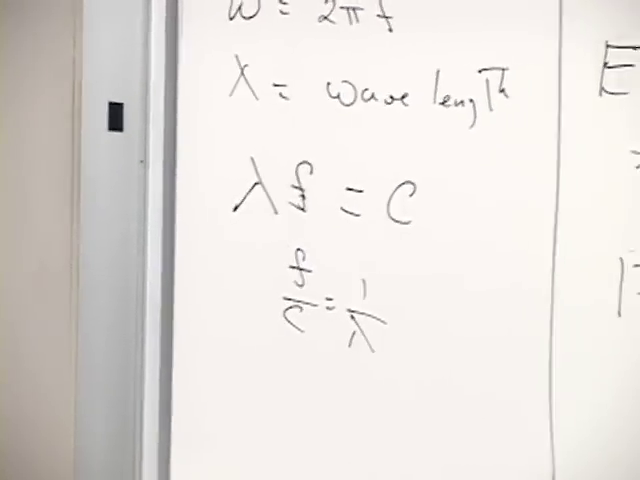
\includegraphics[width=0.56\textwidth]{lecture_02_figure_02.png}
\caption{Для света верны соотношения \(\lambda f=c\) и \(f/c=1/\lambda\), используемые для получения \(|\vec p_\gamma|=h/\lambda\).}
\lectureframe{00:21:39}
\end{figure}

Чем короче длина волны, тем больше импульс фотона. Это один из важнейших квантовых фактов для физики элементарных частиц. Чтобы исследовать малый объект, нужен зонд с короткой длиной волны, и платой за такую короткую длину волны является большой импульс.

\begin{classroomqa}
\lecturetimestamp{00:22:23}
\audiencequestion{Является ли соотношение \(E=\hbar\omega\) фундаментальным, или оно выводится из более глубокого принципа?}
\lecturerresponse{Оно следует из квантовой механики гармонического осциллятора. Здесь этот результат будет использоваться без повторения его доказательства; развиваемый ниже язык осциллятора даёт ему более глубокую основу.}
\end{classroomqa}


\section{Амплитуда волны и число фотонов}

\begin{classroomqa}
\lecturetimestamp{00:23:10}
\audiencequestion{Что означает амплитуда волны в фотонном описании?}
\lecturerresponse{Сравните две волны с одинаковыми длиной волны и частотой, но разными амплитудами, например \(\sin(kx)\) и \(A\sin(kx)\). Классически энергия в фиксированной области пропорциональна квадрату амплитуды. В квантовой механике мода, содержащая \(n\) фотонов, имеет энергию \(n\hbar\omega\). Поэтому при фиксированных частоте, области и нормировке амплитуда по порядку величины растёт как \(\sqrt n\).}
\end{classroomqa}

Эти две волны имеют одинаковую картину колебаний. Одна просто сильнее другой.\footnote{Схема воспроизводит сравнение волн в 00:23:47--00:24:28.}

\begin{figure}[t]
\centering
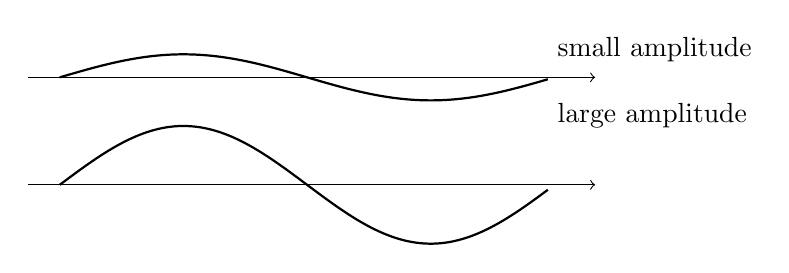
\begin{tikzpicture}[x=1cm,y=0.65cm]
\draw[->] (-0.4,0) -- (6.8,0);
\draw[->] (-0.4,-2.1) -- (6.8,-2.1);
\draw[thick] plot[domain=0:6.2,samples=120] (\x,{0.45*sin(\x r)});
\draw[thick] plot[domain=0:6.2,samples=120] (\x,{-2.1+1.15*sin(\x r)});
\draw (6.2,0.55) node[right]{small amplitude};
\draw (6.2,-0.75) node[right]{large amplitude};
\end{tikzpicture}
\caption{Волны с одинаковыми длиной волны и частотой, но разными амплитудами.}
\end{figure}

При фиксированном количестве волны,
\begin{equation}
E_{\text{wave}}\propto A^2.
\end{equation}
Для электромагнитной волны это знакомое утверждение о том, что энергия поля пропорциональна квадрату напряжённости поля. Если та же мода содержит \(n\) фотонов, то
\begin{equation}
E_{\text{wave}}=n\hbar\omega.
\end{equation}
Следовательно, если зафиксировать моду, частоту, нормировку и область,
\begin{equation}
A^2\propto n\hbar\omega,
\qquad
A\propto\sqrt n\quad\text{at fixed }\omega.
\end{equation}
Здесь не утверждается никакая точная нормировка. Важно, какая часть волны включена: удвоение длины в остальном однородной волны изменяет её полную энергию, не меняя локальной амплитуды. Поэтому пропорциональность можно понимать для фиксированной области, например одной длины волны.

Есть и специфически квантовая оговорка. Амплитуде и фазе нельзя одновременно приписать точные классические значения. Поэтому вопрос ``Какова амплитуда одного фотона?'' неоднозначен, если он требует идеально определённого классического поля. Тем не менее подстановка \(n=1\) даёт разумный масштаб по порядку величины.

\begin{classroomqa}
\lecturetimestamp{00:28:25}
\audiencequestion{Представляет ли вертикальное смещение на рисунке электромагнитной волны положение фотона в пространстве?}
\lecturerresponse{Нет. Ось распространения — пространственная, тогда как вертикальная координата представляет значение электрического или магнитного поля. Импульс направлен вдоль оси распространения, а не вдоль изображённой амплитуды поля.}
\end{classroomqa}

Волна может распространяться в любом пространственном направлении, но на привычном синусоидальном рисунке только горизонтальная ось служит пространственной координатой. Другое изображённое направление показывает величину поля.

\begin{classroomqa}
\lecturetimestamp{00:29:37}
\audiencequestion{Указанное число фотонов считается в пределах одной длины волны или периода волны?}
\lecturerresponse{Можно выбрать фиксированную область, например одну длину волны. Именно поэтому соотношение выражает лишь пропорциональность: полная энергия и число фотонов зависят также от того, какая часть волны включена. Две, три или четыре длины волны содержат соответственно больше энергии, чем одна длина волны при той же амплитуде.}
\end{classroomqa}

\begin{classroomqa}
\lecturetimestamp{00:30:17}
\audiencequestion{Имеет ли смысл амплитуда одного фотона?}
\lecturerresponse{Она имеет смысл только как утверждение о порядке величины, получаемое при подстановке \(n=1\). Для электромагнитной моды информация об электрическом и магнитном полях играет роль, аналогичную информации о сопряжённых координате и импульсе, поэтому квантовая неопределённость ограничивает точность, с которой можно приписать классическую амплитуду. Соотношение по порядку величины остаётся полезным.}
\end{classroomqa}

Эти вопросы уже подводят к квантовой теории поля, где связь между полевыми переменными и числом частиц можно сформулировать точно. Пока достаточно соотношений пропорциональности.

\section{Общие квантовые соотношения и медленные волны вещества}

Некоторые формулы, введённые для фотонов, применимы гораздо шире, а некоторые — нет. Стоит разобраться в них, прежде чем переходить к электронам.

\begin{figure}[t]
\centering
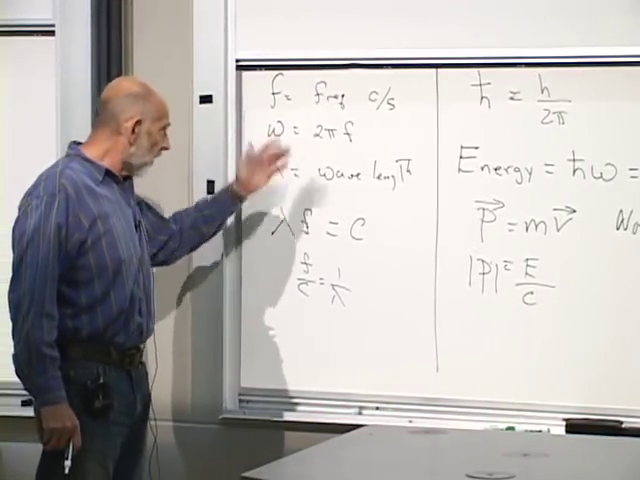
\includegraphics[width=0.82\textwidth]{lecture_02_figure_03.png}
\caption{Определения волн, а также соотношения для фотона и нерелятивистского импульса, сопоставленные по областям применимости.}
\lectureframe{00:31:52}
\end{figure}

Определения \(f\), \(\omega=2\pi f\) и \(\lambda\) применимы в общем случае. Квантовое соотношение
\begin{equation}
E=\hbar\omega=hf
\end{equation}
в рамках настоящего обсуждения тоже является общим. Напротив, формулы, содержащие \(c\), такие как \(\lambda f=c\) и \(|\vec p|=E/c\), применимы к волнам, движущимся со скоростью света. Формула \(\vec p=m\vec v\) применима к частицам, движущимся значительно медленнее света. Для релятивистского движения между этими пределами нужна интерполяция, которая нам пока не требуется.

Соотношение импульса--длины волны сохраняется и за пределами примера с фотоном:
\begin{equation}
p=\frac{h}{\lambda}.
\end{equation}
Здесь \(p\) обозначает модуль, если \(\lambda\) берётся как положительная длина волны; направление можно указать отдельно.

\begin{figure}[t]
\centering
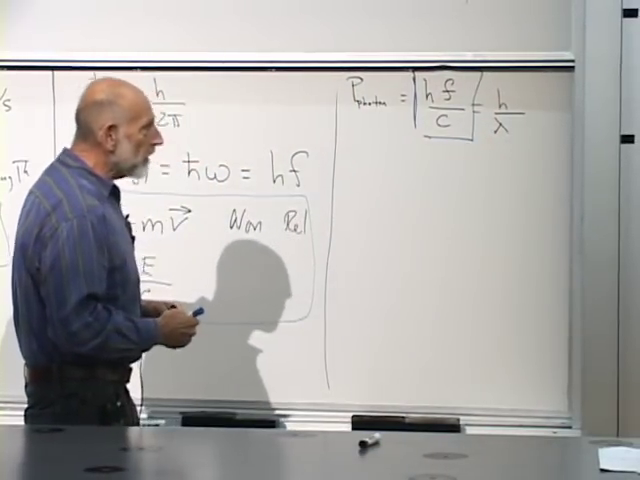
\includegraphics[width=0.74\textwidth]{lecture_02_figure_04.png}
\caption{Импульс фотона \(|\vec p_\gamma|=hf/c=h/\lambda\), из которого следует общее соотношение де Бройля.}
\lectureframe{00:33:32}
\end{figure}

Электрону, ядру и даже шару для боулинга можно сопоставить волну. Интерференция электронов — одно из проявлений этого факта. Запишем электронную волну как \(\psi\). Что заменяет \(\lambda f=c\) для медленно движущегося электрона? Недостающий элемент — нерелятивистское соотношение между энергией и импульсом.

Начнём с кинетической энергии и импульса:
\begin{align}
E&=\frac12 mv^2,\\
p&=mv,
\qquad
v=\frac{p}{m}.
\end{align}
Подстановка последнего соотношения в первое даёт
\begin{align}
E
&=\frac12m\left(\frac{p}{m}\right)^2\\
&=\frac{p^2}{2m}.
\end{align}
Масса стоит в числителе в \(\frac12 mv^2\) и в знаменателе в \(p^2/(2m)\). Это легко перепутать, поэтому полезно вывести это заново.

Теперь используем общие квантовые соотношения
\begin{equation}
E=hf,
\qquad
p=\frac{h}{\lambda}.
\end{equation}
Для одной медленно движущейся частицы
\begin{align}
hf
&=\frac{p^2}{2m}\\
&=\frac{1}{2m}\left(\frac{h}{\lambda}\right)^2\\
&=\frac{h^2}{2m\lambda^2}.
\end{align}
Деление на \(h\) даёт
\begin{equation}
f=\frac{h}{2m\lambda^2}.
\end{equation}

\begin{figure}[t]
\centering
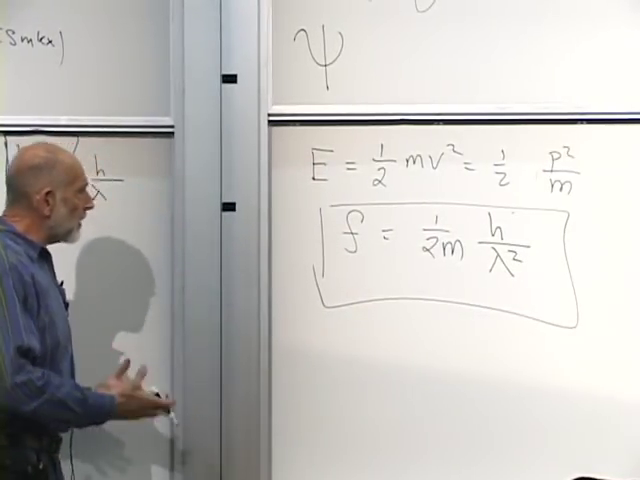
\includegraphics[width=0.64\textwidth]{lecture_02_figure_05.png}
\caption{Для медленной частицы \(E=p^2/(2m)\) и \(p=h/\lambda\) дают \(f=h/(2m\lambda^2)\).}
\lectureframe{00:37:47}
\end{figure}

Для света
\begin{equation}
f\propto\frac{1}{\lambda},
\end{equation}
тогда как для медленного вещества
\begin{equation}
f\propto\frac{1}{\lambda^2}.
\end{equation}
Нет нужды заучивать второе соотношение отдельно. Его всегда можно восстановить из \(E=p^2/(2m)\), \(E=hf\) и \(p=h/\lambda\). Для электрона, медленно движущегося в атоме, оно даёт частоту соответствующей волны Schr\"odinger.

\begin{classroomqa}
\lecturetimestamp{00:38:35}
\audiencequestion{Применимо ли нерелятивистское соотношение частота--длина волны к частицам, отличным от электронов?}
\lecturerresponse{Да. Оно применимо к любой частице, движущейся значительно медленнее света. Релятивистская интерполяция между пределами медленного движения и светоподобного движения — отдельная тема.}
\end{classroomqa}

\begin{classroomqa}
\lecturetimestamp{00:38:55}
\audiencequestion{Какое соотношение применимо к нейтрино?}
\lecturerresponse{Это зависит от скорости нейтрино. Большинство нейтрино, встречающихся в природе, движется очень близко к скорости света, поэтому соотношение для светоподобного случая является хорошим приближением. Нейтрино, движущееся значительно медленнее света, вместо этого подчинялось бы нерелятивистскому соотношению.}
\end{classroomqa}

\editorialnote{Краткий обмен репликами с аудиторией сразу после вопроса о нейтрино касается амплитуд, квантов и различающихся длин волн электронов, но его формулировка слишком сильно повреждена, чтобы её можно было надёжно восстановить. В той части ответа, которую удаётся восстановить, общее соотношение между амплитудами и квантами с разными длинами волн откладывается на потом.}

\begin{classroomqa}
\lecturetimestamp{00:39:56}
\audiencequestion{Электрон из ускорителя \(20\,\mathrm{keV}\) является медленным или релятивистским?}
\lecturerresponse{Его рассматривают как медленный. В единицах с \(c=1\) массу, энергию и импульс можно выражать в одних и тех же единицах. Масштаб энергии покоя электрона равен примерно \(0.5\,\mathrm{MeV}\), тогда как \(20\,\mathrm{keV}\) значительно меньше. Эквивалентно, нерелятивистский критерий для импульса имеет вид \(p\ll mc\).}
\end{classroomqa}

Сравнение энергий в примере имеет вид
\begin{equation}
K=20\,\mathrm{keV}\ll m_ec^2\simeq0.5\,\mathrm{MeV}.
\end{equation}
\editorialnote{В исходном фрагменте 00:39:56--00:41:40 \(20\,\mathrm{keV}\) вводится как энергия ускорителя, а затем релятивистский критерий формулируется в терминах импульса по сравнению с массой покоя. Раздельная запись критериев по кинетической энергии и по импульсу позволяет избежать отождествления приведённой энергии с импульсом, сохраняя при этом сформулированный нерелятивистский вывод.}

\section{Фазовая скорость, групповая скорость и дисперсия}

\begin{classroomqa}
\lecturetimestamp{00:41:46}
\audiencequestion{Можно ли использовать произведение частоты на длину волны, чтобы получить скорость электронной волны?}
\lecturerresponse{Оно даёт фазовую скорость, а не скорость, приписываемую электрону. Локализованный пакет имеет и фазовую скорость, описывающую движение его внутренних гребней и впадин, и групповую скорость, описывающую движение огибающей. Именно групповую скорость отождествляют с движением частицы.}
\end{classroomqa}

Волновой пакет локально похож на синус или косинус, но ограничен огибающей. При движении огибающая и гребни внутри неё не обязаны перемещаться с одной и той же скоростью.\footnote{Схема следует за обсуждением волнового пакета в 00:42:34--00:44:11.}

\begin{figure}[t]
\centering
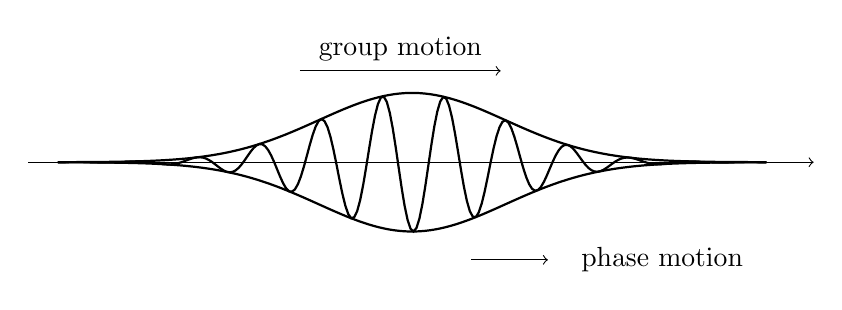
\begin{tikzpicture}[x=0.75cm,y=0.8cm]
\draw[->] (-0.5,0) -- (12.8,0);
\draw[thick] plot[domain=0:12,samples=140] (\x,{1.10*exp(-0.20*(\x-6)^2)});
\draw[thick] plot[domain=0:12,samples=140] (\x,{-1.10*exp(-0.20*(\x-6)^2)});
\draw[thick] plot[domain=0:12,samples=240] (\x,{1.10*exp(-0.20*(\x-6)^2)*sin(6*\x r)});
\draw[->] (4.1,1.45) -- (7.5,1.45);
\draw (5.8,1.8) node{group motion};
\draw[->] (7.0,-1.55) -- (8.3,-1.55);
\draw (8.7,-1.55) node[right]{phase motion};
\end{tikzpicture}
\caption{Локализованный волновой пакет, у которого огибающая и внутренняя фаза в общем случае движутся с разными скоростями.}
\end{figure}

Фазовая скорость — это скорость гребней, впадин и других точек с фиксированной фазой монохроматической компоненты. Для нерелятивистского дисперсионного соотношения,
\begin{equation}
v_\phi=f\lambda=\frac{h}{2m\lambda}.
\end{equation}
она зависит от длины волны. Поэтому компоненты с разными длинами волн имеют разные фазовые скорости, так что гребни могут проходить сквозь пакет, а сам пакет может расплываться. Групповая скорость — это скорость пакета как целого, и именно её отождествляют с движением частицы.

Есть простой частный случай. Если все компоненты с разными длинами волн движутся с одной и той же скоростью, фазовая и групповая скорости совпадают. Свет в вакууме обладает этим свойством: каждая длина волны распространяется со скоростью \(c\). Соотношение для медленной частицы таким свойством не обладает: его \(f\lambda\) меняется с \(\lambda\).

Уравнение
\begin{equation}
f=\frac{h}{2m\lambda^2}
\end{equation}
— это свободное уравнение Schr\"odinger в слегка замаскированном виде. Частота задаёт временную зависимость плоской волны, длина волны — её пространственную зависимость, а уравнение Schr\"odinger связывает их. И наоборот, подстановка волны с определёнными частотой и длиной волны в свободное уравнение Schr\"odinger воспроизводит это дисперсионное соотношение.

\begin{classroomqa}
\lecturetimestamp{00:47:02}
\audiencequestion{Может ли фазовая скорость превышать скорость света?}
\lecturerresponse{Да. Фазовая скорость не переносит информацию. Информация и локализованный пакет распространяются с групповой скоростью, поэтому сверхсветовая фазовая скорость не допускает сверхсветовой передачи сигналов.}
\end{classroomqa}

\section{Конечное пространство и дискретный импульс}

В конечном счёте нас интересуют волны в бесконечном пространстве, но начинать безопаснее с конечной системы. Бесконечность — не то, что компьютер может непосредственно хранить или обрабатывать. Сначала формулируют уравнения для конечной системы и лишь потом переходят к пределу, в котором её размер становится сколь угодно большим. Эта привычка полезна во всей квантовой механике, квантовой теории поля и физике элементарных частиц.

Если начать с одного пространственного измерения, ничего существенного не теряется. Волна может существовать на скрипичной струне, на раскачиваемой верёвке или в абстрактном одномерном мире. Самая очевидная конечная система — это отрезок длины \(L\) с отражающими концами. Волна идёт к концу, отражается и идёт обратно. Это вполне допустимое отражающее граничное условие, но у него есть неудобство: импульс не сохраняется внутри волновой системы. Волна, движущаяся вправо, несёт импульс вправо; после отражения она несёт импульс влево. Граница сообщила системе импульс и поглотила разность.

Изменение знака импульса при отражении на конце можно схематически изобразить.\footnote{Схема следует за рассуждением об отражающей границе в 00:49:24--00:51:08.}

\begin{figure}[t]
\centering
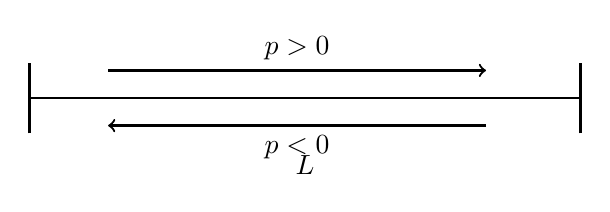
\begin{tikzpicture}[x=1cm,y=1cm]
\draw[thick] (0,0) -- (7,0);
\draw[very thick] (0,-0.45) -- (0,0.45);
\draw[very thick] (7,-0.45) -- (7,0.45);
\draw[->,thick] (1.0,0.35) -- (5.8,0.35) node[midway,above]{\(p>0\)};
\draw[->,thick] (5.8,-0.35) -- (1.0,-0.35) node[midway,below]{\(p<0\)};
\draw (3.5,-0.85) node{\(L\)};
\end{tikzpicture}
\caption{Отражение на концах конечного отрезка обращает импульс бегущей волны.}
\end{figure}

Существует другой способ сделать систему конечной, сохранив при этом импульс. Отождествим два конца отрезка. Результат можно изобразить как окружность, но никакой буквальной окружности, вложенной во второе измерение, не требуется. Математически это означает просто, что координата периодична: пройдя полное расстояние \(L\), мы возвращаемся в ту же точку.

\begin{figure}[t]
\centering
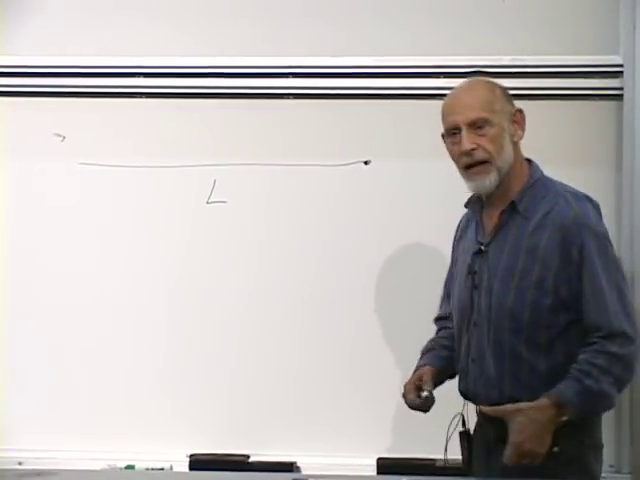
\includegraphics[width=0.72\textwidth]{lecture_02_figure_06.png}
\caption{Одномерный путь полной длины \(L\), используемый для введения периодического отождествления.}
\lectureframe{00:51:21}
\end{figure}

На следующей схеме отождествление концов показано явно.\footnote{Схема следует рассуждению о периодическом отождествлении в 00:51:09--00:52:37.}

\begin{figure}[t]
\centering
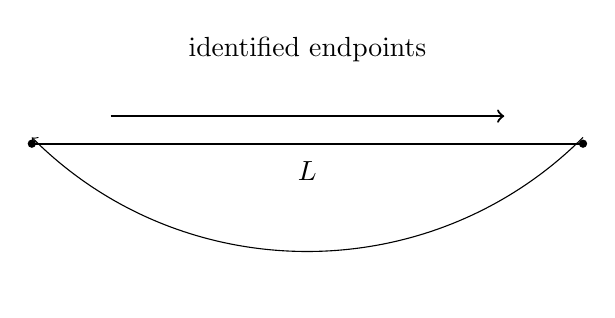
\begin{tikzpicture}[x=1cm,y=1cm]
\draw[thick] (0,0) -- (7,0);
\fill (0,0) circle (1.5pt);
\fill (7,0) circle (1.5pt);
\draw[->,thick] (1.0,0.35) -- (6.0,0.35);
\draw (3.5,-0.35) node{\(L\)};
\draw[->,bend left=45] (7,0.08) to (0,0.08);
\draw (3.5,1.2) node{identified endpoints};
\end{tikzpicture}
\caption{Периодическое одномерное пространство, образованное отождествлением концов пути длины \(L\).}
\end{figure}

Волна, движущаяся вправо, достигает показанного конца, вновь появляется в начале и продолжает двигаться вправо. Волна, идущая влево, аналогично продолжает двигаться влево. Нет выделенного конца, на котором волна отражалась бы, поэтому импульс не меняет знак. Периодическое пространство делает объём конечным и сохраняет импульс, но имеет важное следствие: допустимые импульсы дискретны.

Целое число длин волн должно укладываться в полную длину. Для неконстантной моды,
\begin{equation}
\lambda_{|N|}=\frac{L}{|N|},
\qquad |N|=1,2,3,\ldots .
\end{equation}
Следовательно, длина волны по модулю может быть \(L\), \(L/2\), \(L/3\) и так далее. Вариант вроде \(L/\sqrt{2}\) не подходит: после одного обхода волна вернулась бы с неправильной фазой и не совпала бы со своим начальным значением.

Используя \(p=h/\lambda\), получаем, что модуль импульса для \(|N|\)-й неконстантной моды равен
\begin{equation}
|p_N|=\frac{|N|h}{L}.
\end{equation}
Чтобы без двусмысленности включить оба направления и константную моду, удобно считать, что метка моды может иметь знак:
\begin{equation}
p_N=\frac{Nh}{L},
\qquad N=0,\pm1,\pm2,\ldots .
\end{equation}
Положительные и отрицательные \(N\) соответствуют противоположным направлениям распространения. Мода \(N=0\) постоянна и имеет нулевой импульс; у неё нет конечной длины волны, которую можно было бы подставить в \(h/\lambda\). Поэтому основной шаг по импульсу равен \(h/L\).

При макроскопическом \(L\) и \(h\), и \(1/L\) настолько малы, что этот шаг становится чрезвычайно малым, так что разрешённые значения образуют очень плотное множество и выглядят почти непрерывными. Тем не менее бусинка, движение которой ограничено круговой проволокой, имеет в точности такой дискретный спектр.

\begin{classroomqa}
\lecturetimestamp{00:58:27}
\audiencequestion{Квантованной величиной является полный импульс волны или импульс, связанный с одним периодом?}
\lecturerresponse{Это утверждение относится к импульсу каждого кванта. Каждый квант обладает одним из разрешённых дискретных импульсов. Следовательно, полный импульс любой совокупности квантов также является целым кратным величине \(h/L\).}
\end{classroomqa}

\begin{classroomqa}
\lecturetimestamp{00:59:22}
\audiencequestion{Почему волна после одного обхода должна возвращаться к тому же значению?}
\lecturerresponse{Отождествлённые концы — это одна и та же физическая точка, поэтому наблюдаемое поле должно иметь там одно и то же значение. Несовпадение потребовало бы резкого скачка поля в этой точке. Такой разрыв дорого обходится по энергии и импульсу; допустимые конфигурации поля непрерывны и периодичны.}
\end{classroomqa}

\begin{classroomqa}
\lecturetimestamp{01:00:09}
\audiencequestion{Что происходит, если волна локализована в пакете?}
\lecturerresponse{Пакет представляет собой сумму Фурье плоских волн или, что эквивалентно, синусов и косинусов. В периодическом пространстве эта сумма может содержать только разрешённые дискретные моды импульса. Поэтому утверждение о квантовании есть утверждение о компонентах Фурье любого допустимого пакета.}
\end{classroomqa}

\begin{classroomqa}
\lecturetimestamp{01:01:01}
\audiencequestion{Есть ли проблема, если периодическая длина \(L\) становится чрезвычайно малой?}
\lecturerresponse{По мере уменьшения \(L\) базовый импульс \(h/L\) становится очень большим. Никакого немедленного противоречия на обычных микроскопических масштабах отсюда не следует, но попытка довести эту конструкцию до режима планковской длины, как ожидается, потребует новой физики.}
\end{classroomqa}

Теперь воспримем картину с окружностью буквально: бусинка движется по круговой проволоке радиуса \(r\), длина которой по окружности равна \(L=2\pi r\). Её допустимые тангенциальные импульсы равны
\begin{equation}
p_N=\frac{Nh}{2\pi r}=\frac{N\hbar}{r}.
\end{equation}
Для нерелятивистской частицы на круговой орбите момент импульса равен \(mvr\). Поскольку в этом режиме \(p=mv\), это есть \(rp\). Выражение \(mvr\) не является релятивистски общим, потому что тогда \(p\) уже не равно просто \(mv\), но произведение импульса на перпендикулярное расстояние остаётся правильным соотношением. В векторной форме,\footnote{На лекции сначала для момента импульса используется \(L\), затем обнаруживается его столкновение с \(L\), обозначающим периодическую длину, и обозначение меняется. Здесь повсюду используется \(J\); см. 01:03:40--01:05:21.}
\begin{equation}
\vec J=\vec r\times\vec p,
\end{equation}
и для тангенциального кругового движения его модуль равен \(J=rp\). Следовательно,
\begin{equation}
J_N=rp_N=N\hbar.
\end{equation}
Шаг по линейному импульсу зависит от размера окружности, тогда как единица момента импульса всегда равна \(\hbar\). Когда участвуют фермионы, у правила целочисленности есть исключения; эти исключения пока отложим.

Следующая задача — точнее установить связь между полями, частицами и квантами. Для этого нужно ненадолго вернуться к квантовой механике операторов и гармонического осциллятора.

\section{Волновые моды и квантовые операторы}

Далее квантовая механика неизбежно будет абстрактной и служит повторением. Гармонический осциллятор здесь является основной системой, потому что волна — это колебание. В фиксированной точке электрическое поле, магнитное поле или любая другая волновая амплитуда периодически меняется во времени; сказать, что компонента имеет частоту, уже значит сказать, что она колеблется.

Произвольная волна не обязана иметь только одну длину волны. Свет нескольких цветов может быть смешан, и, наоборот, призма может разложить смешанный свет на составляющие цвета, как в ньютоновском разложении белого света. У каждой компоненты есть собственные длина волны, частота, амплитуда, энергия и импульс. Поэтому смешанную волну можно разложить на кванты с различными энергиями и импульсами. Каждая длина волны определяет частоту, и каждая компонента с определённой частотой ведёт себя как осциллятор. Вот почему естественным строительным блоком для поля является гармонический осциллятор, а не произвольная квантовая система.

Квантовые наблюдаемые представляются операторами. Операторы можно складывать и перемножать, но, в отличие от обычных чисел, их произведения могут зависеть от порядка множителей. Пусть \(A\) и \(B\) представляют два свойства системы, каждое из которых может быть измеримо само по себе. Например, \(A\) может представлять электрическое поле, а \(B\) — магнитное поле. Если измеренные значения — это обычные числа \(a\) и \(b\), то
\begin{equation}
ab=ba.
\end{equation}
Их численное произведение не может зависеть от порядка умножения. Однако в квантовой механике соответствующие операторы могут вместо этого удовлетворять соотношению \(AB-BA\neq0\).

Сначала это кажется бессмысленным. Если измерение электрического поля даёт одно число, а измерение магнитного поля — другое, то произведение этих двух чисел должно давать один и тот же результат в любом порядке. Разгадка в том, что когда произведения операторов зависят от порядка, эти две величины нельзя измерить одновременно. Эксперимент, измеряющий одну из них, вмешивается в измерение другой. Противоречия нет, потому что эти два численных значения нельзя получить совместно.

Когда две величины можно измерить одновременно, их измеренные значения являются обычными числами, и эти числа коммутируют. Поэтому критерием совместной измеримости служит коммутатор
\begin{equation}
[A,B]=AB-BA.
\end{equation}
Нулевой коммутатор означает, что наблюдаемые совместимы; ненулевой коммутатор означает, что соответствующие измерения мешают друг другу. При перестановке аргументов знак меняется на противоположный:
\begin{equation}
[B,A]=-[A,B].
\end{equation}

Для нерелятивистской частицы три компоненты положения коммутируют друг с другом, и то же верно для трёх компонент импульса:
\begin{align}
[x,y]&=[y,z]=[z,x]=0,\\
[p_x,p_y]&=[p_y,p_z]=[p_z,p_x]=0.
\end{align}
Все три координаты можно задать одновременно, и все три компоненты импульса тоже можно задать одновременно. Соответствующие компоненты положения и импульса не коммутируют:
\begin{equation}
[x,p_x]=[y,p_y]=[z,p_z]=i\hbar,
\end{equation}
тогда как смешанные компоненты, такие как \([x,p_y]\), равны нулю. Измерение координаты сообщает частице возмущение в сопряжённом импульсе. Эквивалентно, произведение неопределённостей соответствующих координаты и импульса определяется величиной \(\hbar\).

\begin{classroomqa}
\lecturetimestamp{01:16:30}
\audiencequestion{При переходе от \(x\) к \(y\), должно ли \(i\) в коммутаторе измениться на \(j\)?}
\lecturerresponse{Нет. Символ \(i\) всегда обозначает мнимую единицу, квадратный корень из минус единицы. Он не является ни меткой декартова единичного вектора, ни одним из кватернионных символов \(i,j,k\).}
\end{classroomqa}

\begin{classroomqa}
\lecturetimestamp{01:17:24}
\audiencequestion{Означает ли \(AB-BA\), что сначала измеряется \(A\), затем \(B\), а потом порядок измерений меняется на обратный?}
\lecturerresponse{Нет. Эти два члена представляют собой произведения операторов или матриц, взятые в разных алгебраических порядках. Они не обозначают буквальную последовательность измерений. Связь с несовместимыми измерениями является следствием алгебры операторов, а не определением произведения.}
\end{classroomqa}

\begin{classroomqa}
\lecturetimestamp{01:18:32}
\audiencequestion{Эти коммутаторы координаты--импульса непосредственно применимы к фотону?}
\lecturerresponse{Не напрямую. Они без оговорок применимы к нерелятивистским частицам. Координату фотона определить труднее, поэтому аналогичное утверждение требует большей осторожности и здесь не нужно.}
\end{classroomqa}

\section{Квантовый гармонический осциллятор}

Груз на пружине, звуковая волна и световая волна — все это примеры колебательного движения. У всякого идеального гармонического осциллятора есть частота. Для пружины один полный период — это не просто время, за которое груз возвращается в то же положение; он должен вернуться в это положение, двигаясь в том же направлении. Число полных периодов в секунду есть \(f\), а \(\omega=2\pi f\).

Классически идеальный осциллятор может иметь любую неотрицательную энергию. Легкий толчок сообщает небольшую энергию, а более сильный — большую. Настоящая пружина в конце концов сломалась бы или расплавилась, но в математической идеализации существует непрерывный диапазон положительных энергий. Квантовый осциллятор устроен иначе: его допустимые энергии образуют дискретную равноотстоящую лестницу. Выбирая начало отсчета энергии так, чтобы нижний уровень назывался нулем,
\begin{equation}
E_n=n\hbar\omega,
\qquad n=0,1,2,\ldots .
\end{equation}
Равноотстоящие уровни можно изобразить следующим образом.\footnote{Схема энергетических уровней следует обсуждению у доски в 01:21:20--01:23:56.}

\begin{figure}[t]
\centering
\begin{tikzpicture}[x=1cm,y=0.9cm]
\draw[->] (0,0) -- (0,5.35);
\draw (0,5.5) node[above]{energy};
\foreach \y/\lab in {0.6/{0},1.6/{\hbar\omega},2.6/{2\hbar\omega},3.6/{3\hbar\omega},4.6/{n\hbar\omega}}
{
  \draw[thick] (0.2,\y) -- (2.2,\y);
  \draw (-0.25,\y) node[left]{\(\lab\)};
}
\draw[->,thick] (2.8,0.68) -- (2.8,1.52);
\draw (3.2,1.1) node[right]{\(a_+\)};
\draw[->,thick] (3.7,1.52) -- (3.7,0.68);
\draw (4.1,1.1) node[right]{\(a_-\)};
\end{tikzpicture}
\caption{Равноотстоящие уровни осциллятора в соглашении \(E_n=n\hbar\omega\).}
\end{figure}

Интервал \(\hbar\omega\) — это та же энергия, которая ранее была приписана одному фотону с угловой частотой \(\omega\). Величина \(2\hbar\omega\) может быть энергией одного кванта, принадлежащего осциллятору с частотой \(2\omega\), или энергией двух квантов в осцилляторе с частотой \(\omega\). Здесь нужна вторая интерпретация. Один осциллятор фиксированной частоты может содержать ноль, один, два, три или больше квантов, и между ступенями никаких допустимых энергий нет.

Целое число \(n\) помечает состояние осциллятора, записываемое как кет \(|n\rangle\). Состояние \(|0\rangle\) есть основное состояние, \(|1\rangle\) содержит один квант возбуждения, \(|2\rangle\) — два и так далее. Кет — это просто обозначение состояния, на которое действуют операторы.

Определим оператор повышения \(a_+\), который переводит состояние на один уровень вверх, и оператор понижения \(a_-\), который переводит его на один уровень вниз:
\begin{align}
a_+|n\rangle &= \sqrt{n+1}\,|n+1\rangle,\\
a_-|n\rangle &= \sqrt{n}\,|n-1\rangle.
\end{align}
Числовые множители с квадратными корнями входят в определения. Для самого нижнего состояния
\begin{equation}
a_-|0\rangle=0,
\end{equation}
поскольку ниже основного состояния нет никакого состояния.

Здесь важно различать обычные числа и операторы. Метка \(n\) и коэффициенты, такие как \(\sqrt n\), являются обычными числами; они коммутируют со всем. Символы \(a_+\) и \(a_-\) — операторы, и их порядок должен сохраняться.

Сначала понизим \(|n\rangle\), а затем снова повысим его. Шаг понижения дает
\begin{equation}
a_-|n\rangle=\sqrt n\,|n-1\rangle.
\end{equation}
Действие \(a_+\) на полученное состояние дает еще один множитель \(\sqrt n\), потому что повышение \(|n-1\rangle\) возвращает его в \(|n\rangle\):
\begin{align}
a_+a_-|n\rangle
&=a_+\bigl(\sqrt n\,|n-1\rangle\bigr)\\
&=\sqrt n\,\sqrt n\,|n\rangle\\
&=n|n\rangle.
\end{align}
Таким образом, \(a_+a_-\) считывает номер уровня. Например, пусть известно, что \(|\chi\rangle\) является собственным состоянием оператора числа, но метка его уровня неизвестна. Если
\begin{equation}
a_+a_-|\chi\rangle=q|\chi\rangle,
\end{equation}
то обычный числовой коэффициент \(q\) есть число квантов в этом состоянии. Следовательно, это произведение есть оператор числа,
\begin{equation}
\hat n=a_+a_-,
\end{equation}
а в выбранном соглашении об энергии гамильтониан равен
\begin{equation}
H=\hbar\omega\,a_+a_-.
\end{equation}
Действительно, при действии на любой уровень получается \(H|n\rangle=n\hbar\omega|n\rangle\).

Теперь поменяем порядок. Сначала повышение дает \(\sqrt{n+1}|n+1\rangle\). Затем понижение возвращает к \(|n\rangle\) и дает второй множитель \(\sqrt{n+1}\):
\begin{align}
a_-a_+|n\rangle
&=a_-\bigl(\sqrt{n+1}\,|n+1\rangle\bigr)\\
&=\sqrt{n+1}\,\sqrt{n+1}\,|n\rangle\\
&=(n+1)|n\rangle.
\end{align}
Эти два порядка отличаются на единицу на каждом состоянии, поэтому
\begin{equation}
[a_-,a_+]=a_-a_+-a_+a_-=1.
\end{equation}

У осциллятора есть также амплитуда и фаза. Его фаза задает, в каком месте цикла он находится; конкретно, ее можно зафиксировать моментом времени, в который осциллятор проходит через начало координат в выбранном направлении. Если задержать это прохождение, фаза изменится без изменения частоты. Операторы повышения и понижения объединяют квантовые переменные, связанные с амплитудой и фазой. Их алгебра по своей природе квантовая, но их действие просто: \(a_+\) добавляет один квант энергии осциллятора, а \(a_-\) удаляет один. Для электромагнитной моды эти кванты являются фотонами, поэтому эти два оператора называются операторами рождения и уничтожения.

\begin{classroomqa}
\lecturetimestamp{01:37:34}
\audiencequestion{Соответствуют ли операторы повышения и понижения физическому измерению?}
\lecturerresponse{Число фотонов измеримо. Операторы \(a_+\) и \(a_-\) по отдельности не являются измеримыми наблюдаемыми по дополнительным техническим причинам. Их коммутатор показывает, что эти два оператора не коммутируют, но сам по себе этот факт не является аргументом в пользу того, что любой из них по отдельности не может быть наблюдаемой величиной.}
\end{classroomqa}

Набор пружин с различными собственными частотами дает много независимых осцилляторов. То же верно и для электромагнитных мод в полости: одна длина волны может быть возбуждена без требования, чтобы остальные имели такое же возбуждение. Квантовомеханически операторы рождения и уничтожения добавляют и удаляют кванты фиксированной частоты в каждом независимом осцилляторе. Этот язык является центральным, потому что частицы будут отождествлены именно с этими квантами.

\section{Поле как совокупность осцилляторов}

Вернемся к периодическому одномерному пространству полной длины \(L\). Его непостоянные моды имеют модули длин волн
\begin{equation}
\lambda_N=\frac{L}{N},
\qquad N=1,2,3,\ldots ,
\end{equation}
и соответствующие неотрицательные угловые частоты \(\omega_N\). Для сравнения с ранее обсуждавшимся спектром импульса удобно обозначить соответствующее целое число со знаком через \(M\):
\begin{equation}
p_M=\frac{Mh}{L},
\qquad M=0,\pm1,\pm2,\ldots .
\end{equation}
Знак \(M\) указывает направление распространения.
\editorialnote{В 01:42:08--01:42:24 индекс частотной моды исправлен: вместо диапазона со знаком используется диапазон, идущий от нуля вверх. Символ \(M\) используется здесь только для того, чтобы отделить обозначение знакового импульса от неотрицательной метки частотной моды \(N\); он не вводит независимых чисел заполнения для \(+M\) и \(-M\). Список непостоянных осцилляторов начинается с \(N=1\).}

Каждая допустимая частота ведет себя как гармонический осциллятор. Энергию можно независимо добавить сначала одной частоте, а затем другой. Подробный первый пример квантового поля отложен до следующей лекции, но обозначение состояний уже ясно. Располагая непостоянные моды, начиная с наибольшей длины волны, запишем
\begin{equation}
|n_1,n_2,n_3,\ldots\rangle,
\end{equation}
где \(n_N=0,1,2,\ldots\) — число квантов в осцилляторе с частотой \(\omega_N\). Первый элемент показывает, сколько квантов занимает моду с наибольшей длиной волны, второй — сколько занимает следующую моду, и так далее без конца.

Гармоники струны делают эту конструкцию наглядной. Переход от основной гармоники к двум следующим показан схематически.\footnote{Схема следует обсуждению гармоник струны в 01:45:20--01:47:46.}

\begin{figure}[t]
\centering
\resizebox{\linewidth}{!}{%
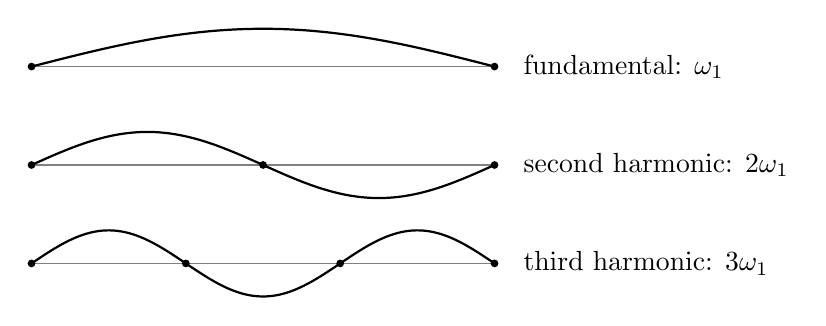
\begin{tikzpicture}[x=0.98cm,y=1cm]
\draw[gray] (0,2.5) -- (6,2.5);
\draw[thick] plot[domain=0:6,samples=120] (\x,{2.5+0.48*sin(30*\x)});
\fill (0,2.5) circle (1.4pt);
\fill (6,2.5) circle (1.4pt);
\node[right] at (6.25,2.5) {fundamental: \(\omega_1\)};

\draw[gray] (0,1.25) -- (6,1.25);
\draw[thick] plot[domain=0:6,samples=120] (\x,{1.25+0.42*sin(60*\x)});
\fill (0,1.25) circle (1.4pt);
\fill (3,1.25) circle (1.4pt);
\fill (6,1.25) circle (1.4pt);
\node[right] at (6.25,1.25) {second harmonic: \(2\omega_1\)};

\draw[gray] (0,0) -- (6,0);
\draw[thick] plot[domain=0:6,samples=120] (\x,{0.42*sin(90*\x)});
\fill (0,0) circle (1.4pt);
\fill (2,0) circle (1.4pt);
\fill (4,0) circle (1.4pt);
\fill (6,0) circle (1.4pt);
\node[right] at (6.25,0) {third harmonic: \(3\omega_1\)};
\end{tikzpicture}%
}
\caption{Основная гармоника струны и ее вторая и третья гармоники с нулем, одним и двумя внутренними узлами.}
\end{figure}

Основная гармоника колеблется в виде одной широкой дуги и не имеет внутренних узлов. Это один осциллятор, и он может содержать \(n_1=0,1,2,\ldots\) квантов; каждое возбуждение требует \(\hbar\omega_1\). Вторая гармоника имеет один внутренний узел и вдвое большую частоту. Если основная гармоника звучит как до первой октавы, то эта мода звучит как нота до на октаву выше. Она имеет независимое число заполнения \(n_2\), и каждый ее квант требует \(\hbar\omega_2=2\hbar\omega_1\). Третья гармоника имеет два внутренних узла и втрое большую частоту, чем основная. Она имеет собственное независимое число заполнения \(n_3\), которое снова может быть любым неотрицательным целым числом.

Для каждой моды, в использованном выше соглашении об энергии, энергия равна числу заполнения, умноженному на энергию кванта. Собрав эти вклады, получаем
\begin{equation}
E=\sum_{N=1}^{\infty} n_N\hbar\omega_N.
\end{equation}
\editorialnote{Эта выписанная сумма представляет собой алгебраическое объединение энергий мод, сформулированных по отдельности в 01:44:02--01:47:46.}

Одну и ту же математику гармонического осциллятора нужно повторить для каждой моды поля, по одному оператору рождения и одному оператору уничтожения для каждого независимого осциллятора. В этой первой элементарной картине квантовое поле — это вся эта совокупность осцилляторов и их алгебра рождения--уничтожения.

Этот язык приспособлен к рассеянию частиц. В эксперимент входят кванты с определёнными энергией и импульсом, а выходят из него кванты с другими энергиями и импульсами. Начальные частицы удаляются операторами уничтожения; вылетающие частицы вводятся в конечное состояние операторами рождения соответствующих мод.

\begin{classroomqa}
\lecturetimestamp{01:49:38}
\audiencequestion{Используется ли одно и то же целое число и для обозначения моды осциллятора, и для подсчёта числа квантов в ней?}
\lecturerresponse{Имеются два различных целых числа. Метка моды \(N\) задаёт пространственную форму; в примере со струной число её узлов определяет частоту \(\omega_N\). Число заполнения \(n_N\) указывает, сколько имеется квантов с этой частотой.}
\end{classroomqa}
